% Design Development 
\chapter{设计开发}
\label{sec-development}

\begin{remark}  \color{blue}
\begin{itemize}\tightlist
\item The design is the protagonist of the story; the design team is only a supporting character. 
\item Focus on results (e.g., key findings, insights, lessons learned), not activity (``We brainstormed extensively and eventually settled on two alternative concepts.'')
\item Use lots of images, and not just photographs: diagrams, schematics, flow charts, CAD renderings, etc. are often much more informative than a photo. In any case, use labels pointing to the features you want the reader to appreciate.
\item Lengthy details (e.g. detailed results of technical benchmarking) should go in an Appendix section, with an explicit forward reference from this section.
\item Be professional: for benchmarking, it's essential to properly cite sources of information and provide credits for any images you are using that you did not generate yourselves.
\item Don't refrain from describing ideas that were briefly pursued and dropped. Explain why they were abandoned. In other circumstances they might be worth picking up again.
\item You can use tools such as Pugh concept selection, function-structure diagrams and design decomposition to organize and clarify your design process \cite{Otto07,OttoWood01,UlrichEppinger95}.
\end{itemize}
\normalcolor 
The remaining text in this section contains of excerpts from the Autodesk 2007-08 Fall document \cite{Autodesk2008Fall}.
\end{remark}

首先我们对市场上现有的远程呈现机器人做了一些调查比较。

\begin{figure}[h]
        \begin{center}
                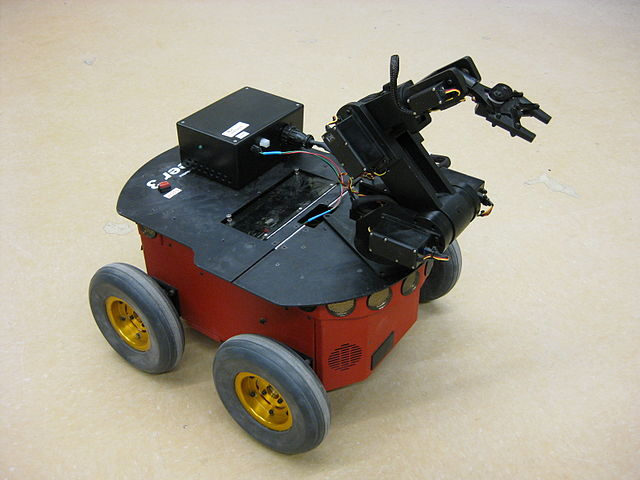
\includegraphics[keepaspectratio, width=4in]{Figures/ch4.our.jpg}
        \caption{AT-3机器人,将来它会变成什么样子?}
        \end{center}
        \label{fig:Design_Development_Flowchart}
\end{figure}

% \section{Brainstorming}
% \label{sec:brainstorm}

%       Our experience in brainstorming was unique in that we were observing and studying our own behavior while exploring solutions. We were constantly studying our own triumphs and shortcomings in the hopes of gaining insight into team dynamics. The results of our multiple brainstorms throughout the fall quarter can be into categorized the following categories:

% \subsection{Communication}

% \begin{figure}[h] 
%       \begin{center}
%               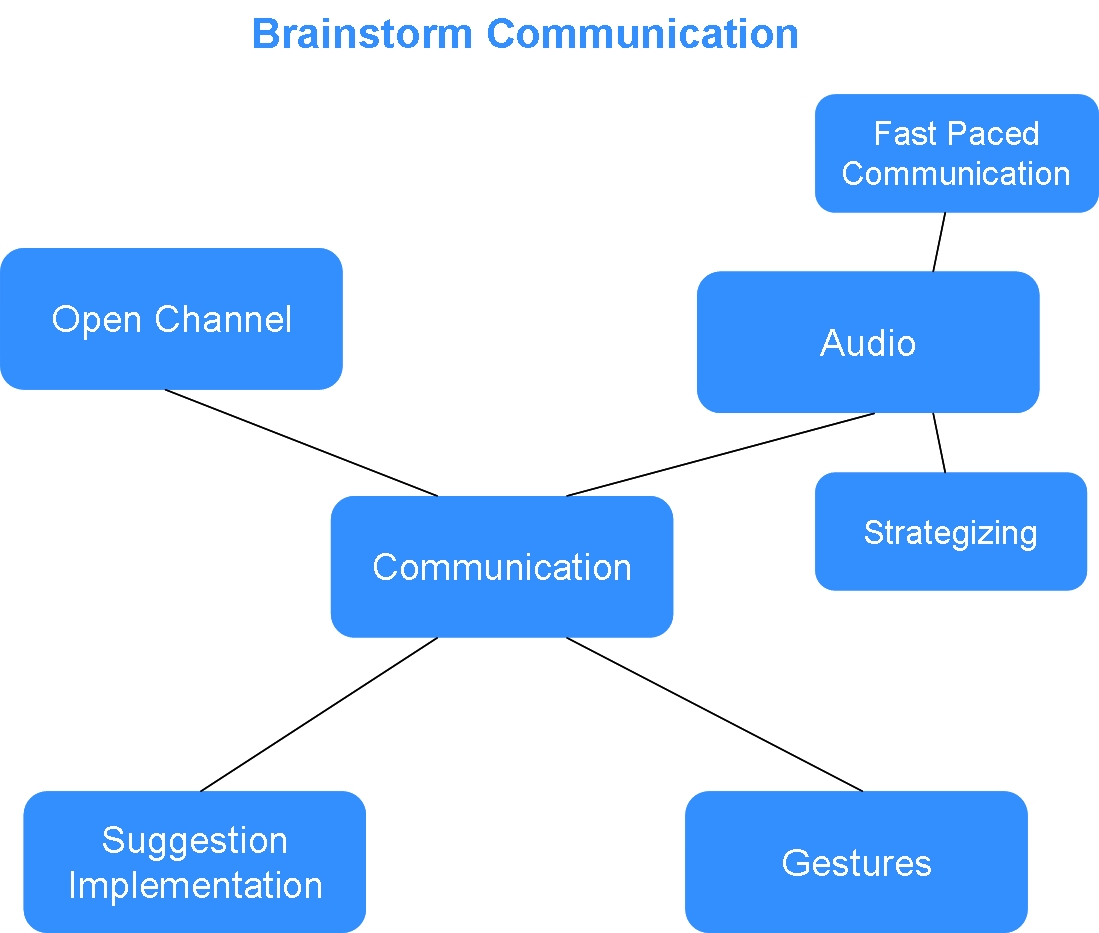
\includegraphics[keepaspectratio, width=3in]{Figures/Ch4/Brainstorm_Communication.jpg}
%       \caption{Key components of communication in design meetings}
%       \label{fig:Brainstorm_Communication}
%       \end{center}
% \end{figure}

% \begin{itemize} \tightlist 
% \item {Open channels}
% \item \begin{itemize} \tightlist Audio and video channels are often inundated with information, even if they are not the most effective means to transmit a piece of information. The team learned that messages are most clearly conveyed when they are free from interference. \end{itemize}
% \item Integrate suggestions quickly
% \item \begin{itemize} \tightlist People can build onto other's ideas immediately, and rapidly change the direction of the conversation. \end{itemize}
% \item \textbf{Verbal communication is the most flexible}
% \item \begin{itemize} \tightlist The team learned from their experience playing cutting-edge multiplayer videogames that verbal communication was the most relied upon medium during fast and slow paced activities. It's versatility and low-bandwidth warranted future attention. \end{itemize}
% \item Gesture
% \item \begin{itemize} \tightlist Gesture is frequently used when explaining an idea. Often, the drawings produced do not look at all like the concept being developed, but the act of drawing in and of itself can be like a gesture, showing how something will work, or where it will be placed, and so forth. \end{itemize}
% \end{itemize}

% \begin{center}
% \color{blue}
% The rest of this subsection is omitted for brevity
% \normalcolor
% \end{center}

% Some key realizations from the brainstorming phase were that social factors and communication shortcomings had alot of opportunity for development. We decided to give special attention to social benchmarking in addition to our technological research.

\section{调查与评估}

市场上已经有将远程呈现机器人技术产业化的例子,但它们的应用似乎都还不广
泛。

\subsection{RP-7i}

\begin{figure}[h] 
\centering
                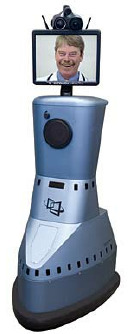
\includegraphics[keepaspectratio, width=2in]{Figures/ch4.rp7i.jpg}
%Note the use of a short caption tag for the list of figures.
        \caption[RP-7i]{RP-7i医疗服务机器人。价格:50000\$/年\textregistered.}
\end{figure}

我们在IEEE的一片综述中发现了这款机器人。它的使用价格很昂贵,但功能并不
出众,它仅能被医生控制着去检查病人。

\noindent \textbf{关键收获}
\begin{itemize} \tightlist
\item  价格是必须考虑的关键因素。高昂的售价应该是远程机器人不普及的一
  个原因。这也启发了我们将远程呈现机器人作为公共服务提供给广泛的人群免
  费使用。
\end{itemize}

\subsection{TEXAI}

Willow Garage公司是智能机器人领域内的先锋,其推出的TEXAI机器人也是功能
强大。这一点在美剧The Big Bang Theory第四季第二集中得到了充分的展现。

\begin{figure}[h] 
\centering
                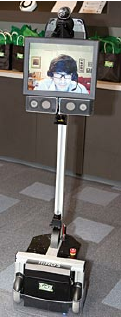
\includegraphics[keepaspectratio, width=2in]{Figures/ch4.texai.jpg}        
%Note the use of a short caption tag for the list of figures.
        \caption[TEXAI]{TEXAI \textregistered 是由Willow Garage公司推
          出的一款远程呈现机器人.}
\end{figure}

\noindent \textbf{关键收获}
\begin{itemize} \tightlist
\item  方便的操控性和灵活美观的外观是一款好的设计的必备要素。
\end{itemize}

\section{关键体验原型 (CEP)}

综合之前的需求调查以及基准测试所得到的结果,我们对于远程呈现机器人所
带给使用者的体验原型的进行了初步的确定。其中,通过头脑风暴以及部分试用受访
者的建议,我们总结出了几个比较突出的方面,用以优化CEP。

\subsection{现况}

我们所拥有的基础是一台可以接受上位机指令进行运动动作的移动机器人,为使其能够成为用用户体验使用的远程呈现机器人,需要将指令的发送方从本地抽离,并通过网络传输到达本地,让机器人拥有此项基本功能是进行用户体验测试的基础。

\subsection{起步}

对于搭建关键体验模型的构造与测试基础,我们选取了网页的形式作为操作界面的具体呈现,之所以采用如此形式,是考虑到了网页的诸多优势,比如:网页可以跨平台使用,可移植性较好,页面对于用户的呈现简单,免去了客户端安装等的前缀过程,简洁可靠。

\section{锁定使用者所关注的方面}

通过用户对机器人简单地试用,我们记录了一些条目,用于CEP决策的主要方面。

\subsection{测试与决策}

\begin{enumerate}

\item 控制方式:对于机器人的操作是嵌入网页中的,就其具体实现形式是多样的,比如页面上的按钮点击出发操作指令的下达,键盘上方向键触发操作指令下达。在使用者测试中,当使用者了解到了方向键的控制的可行性后,便会自然地忽略了页面上布置的按钮。

如上结果应该源自移动类物体的方向属性,以及人类本质属性所决定的形象化归类。

\begin{figure}[bht]

  \centering

  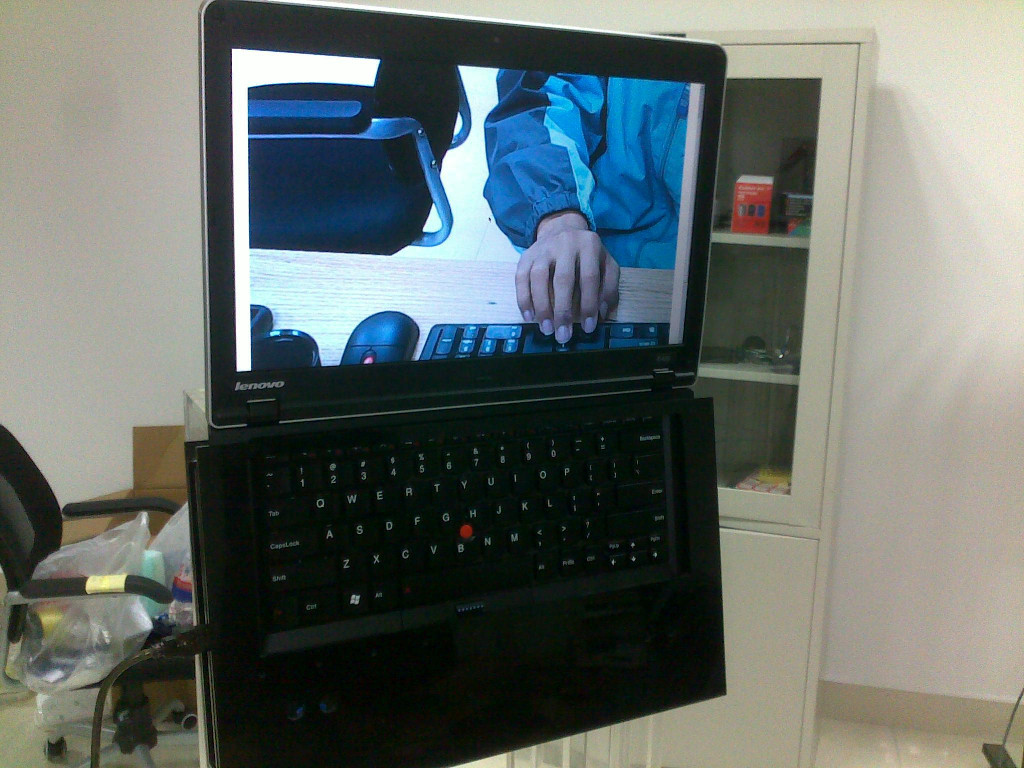
\includegraphics[height= 9cm]{Figures/control.pdf}

\end{figure}


\item 稳定性:最原始的测试模型中,远程呈现机器人端的上位机(笔记本电脑)是固定在机器人的最上方,这是最简单的考虑到屏幕位置与人的舒适性所导向的,但是在测试过程中,由于上层支架的高度较高,以及其连接处的稳固性并非十分理想,机器人在移动加速度较大的时候,上位机端的震动会变得十分明显,如果机器人视觉传感也固定在此处的时候,会对画面的品质造成较大的影响。

测试结果,可以更换上位机的目前的状态,比如在支架的高处仅安置用以人机交互的轻质的显示设备,而将上位机重心下移,这一观点的正确定在随后的测试中也得到了一定的验证,将笔记本电脑放置在下部(移动机构附近),即使有较大的移动加速度,上层结构也会有较好的稳定性。

\item 机器人视角:用于测试的视觉传感器为普通的网络摄像头,由于其视角范围较为狭小,无法同时获得近距离路面状况以及前方环境状况的信息,使得操作时给人的感觉并非十分自然。

测试结果,单一简单地摄像头并不能较好的模拟人类的视角,可以在摄像头上附加转动机构,优化视角的范围;另一个解决方案是,使用广角摄像头完成影像的采集。

\item 视觉功能:仅仅完成视觉的传输呈现是最基本的要求,可以在页面上集成一些如图像抓取、视频录制等的附加功能。

\end{enumerate}
        
% \subsubsection{Tactile CFP Concept Development}

% The team wanted to come up with a creative solution that would enhance distance communication. Although we identified software having an important role in our solution, we wanted to try to design something physical. We had to answer these questions that were raised after the benchmarking process:
% \begin{itemize} \tightlist
% \item How can we simulate proximity for remote meetings?
% \item How can we implement action-event control?
% \item What senses can we stimulate that aren't normally used?
% \item What is a low bandwidth solution?
% \end{itemize}

%         The team decided that building a tactile messaging system would solve all four of the aforementioned questions. Tactile messages could replace common interpersonal interaction found in same room meetings. It is normal to welcome each other with a  handshake, make eye contact throughout a meeting, smile at each other, and give high-fives to congratulate others. These occurrences are all absent from distance meetings. A tactile message corresponding to each of these gestures would allow users similar opportunity to communicate as if they were sharing the same physical meeting room.
        
%         The team learned that immersive activities like videogames take advantage of action-event control to offer users a seamless means to interact with their environment. A tactile message could quickly be sent over an open channel and pressing the on button would instantly message the recipient.
        
%         Out of the five senses (sight, hearing, taste, touch, and smell), sight and hearing are the most relied upon during meetings. The team considered possibilities in taste and smell messaging but continued with touch, since delivery of tactile messaging was much more straightforward. Since conventional distance meetings only send and receive auditory and visual information, tactile messages would be distinct and easy to identify. The team believed that tactile messages (high, low, or off) would be low bandwidth.

%         \begin{figure}[h] 
% \centering
%                 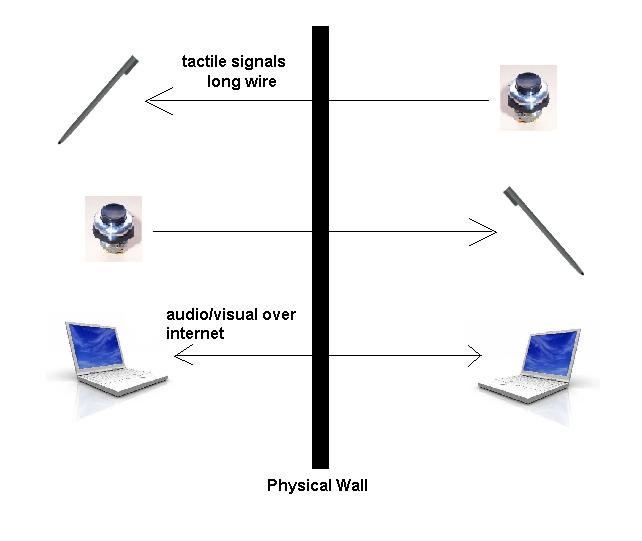
\includegraphics[keepaspectratio, width=4in]{Figures/Ch4/tactileCFPschematic.jpg}
%         \caption{The team's whiteboard during a brainstorm session}
% \end{figure}

%         The team wanted to test the effectiveness of tactile messaging and decided against a TCP/IP protocol that sent messages between Stanford and PUJ. The code to write such a protocol was extant and it was unnecessary to include it in our prototype. The team simplified the setup and created two stations separated by physical barriers (a wall and 50' of distance), to simulate a distance meeting. Each station would have a vibrating tactile device for each seated participant at that station and a high/low button assembly to activate the vibrating tactile device for each participant at the other station. Initially the devices were supposed to operate as ''on'' or ''off.'' The team decided that having more variability in the operating speeds of the motors would increase the number of different messages that could be sent, and added a high and low voltage button (1.2V and 0.6V).
%         We were curious to see if effective communication could take place if a distant colleague could see what sketches his distant colleague was drawing. To test this, we used webcams to send live video of what the participants drew on their drawing pads to the other stations.

% \subsubsection{What is critical about this CFP?}
%         The team identified these questions as critical before testing:
% \begin{enumerate} \tightlist
% \item Can it create immersion?
% \item Does it improve upon existing communication tools?
% \item Is it easy to understand?
% \item Is it intuitive?
% \item When should it be used?
% \end{enumerate}

% \begin{figure}[h] 
%         \begin{center}
%                 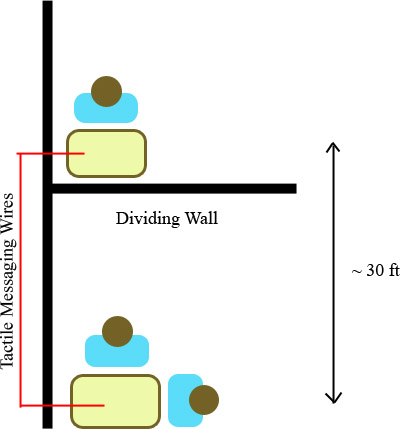
\includegraphics[width=3in]{Figures/Ch4/tactile_seating.jpg}
%         \caption{The orientation of the two tactile messaging stations.}
%         \end{center}
% \end{figure}

% %A transcript of the meeting with tactile feedback is available in Appendix \ref{sec:tactiletranscript}.

% \subsubsection{Lessons Learned}

%         Tactile sensation is an effective means of communicating contextual information. The messaging system delivered instant vibration between the two stations, helping preserve the flow of conversation without impeding it. Using the vibrations to alert the other users that you wanted to say something was a good way to make comments at the precise time you intended. The tactile devices were \textbf{easy to use} and the participants were encouraged to use them as they saw fit. We noticed that \textbf{vibrations were used most frequently to add emphasis} to accompany laughter, to confirm agreement, offer praise for a good idea and to interrupt the speaker. Interruptions consisted of calls for clarification on a point raised or disagreement with an opinion. Interrupting someone who is speaking can cause the speaker to lose his train of thought or become otherwise agitated. We noticed that \textbf{users preferred to send low speed vibrations} as a gentle interruption as a first attempt to get the speaker's attention. If the first few low speed vibrations did not stop the speaker, the high speed vibrations could be sent, and these usually registered right away. We observed that users reserved high speed vibrations for urgent or important messages. 
        
        
%         The signals were mostly easy to detect, but it was \textbf{not always clear what those signals were trying to communicate}. Ambiguous or superfluous signals distracted the receiving user from the meeting and the confused user would ask, ''Did you just buzz me?'' or ''Why did you buzz me?'' These confused questions would stall the meeting for everyone until the sender was revealed and was able to explain what they were trying to communicate. 
        
%         Vibrations, however, were easily detectable despite loud side conversations, a party in a neighboring room, and constant distractions from people walking by. We attribute this to the fact that the tactile channel is uncrowded compared to the audio channel. In a loud environment it is difficult to pick out audio communication from Skype. Visual distractions make it difficult to focus on the laptop monitor. The tactile sensation rarely stimulated in a teleconference, thus making the slightest vibration very noticeable. 
        
%         We tried two different vibrating interfaces, a vibrating pen and a vibrating wrist patch. The wrist patch was unanimously rejected by the participants because 1) the double stick tape that connected the patch to the user's skin was either too sticky and removed arm hair or not sticky enough after a few uses and would fall off, 2) was tethered to the power supply and restricted movement to the point where the hand with the patch was essentially stationary, 3) vibrations on your wrist are not comfortable, and 4) worry that the patch might give the user an electrical shock. The pen had a practical use, writing, and although the pen was connected to the power supply, the user was not, and the range of motion was adequate enough to write anywhere on the drawing space.
        
%         We finally compared the tactile messaging conference to previous experiences with video conferencing and audio conferencing. These results are summarized in Appendix \ref{sec:Appendix1}.
        
%                 \begin{figure}[h] 
% \centering
%                 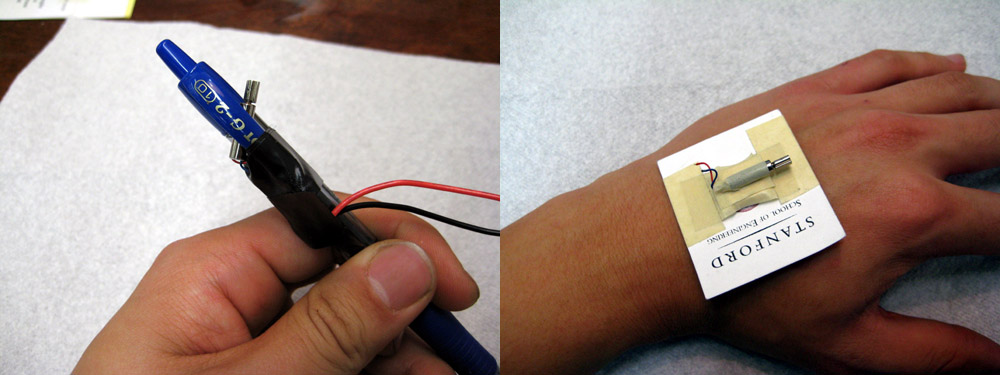
\includegraphics[width=0.8\textwidth]{Figures/Ch4/tactile_motor.jpg}
%         \caption[Messaging station wires]{The orientation of the two tactile messaging stations. (Note: the wires connecting the patch to power supply are not in this photo)}
% \end{figure}

%         The tactile messaging critical function prototype was a success in that it definitively answered all the critical questions we asked ourselves before testing.
